\section{Evolució temporal de l'API}

    \subsection{Evolucions al llarg del temps}

    \paragraph{}
    L’API de FamilySearch s’ha vist subjecte a diversos canvis i modificacions al llarg del temps, algunes, amb més repercussió i implicacions que altres. La llista de canvis és prou llarga com per no intentar reproduir-la en la memòria, però de totes maneres, en cas de curiositat, aquesta s'adjunta a la bibliografia del projecte\footfullcite{fs:apiChangeLog}.

    Cal tenir en compte que l'API de FamilySearch està en constant evolució i que per tant, qualsevol canvi inesperat, pot trencar i interferir en la planificació de qualsevol projecte informàtic que l'utilitzi. Aquest mateix aspecte va provocar, que la pausa realitzada entre els dos intents de realització del projecte, fes que la feina prèvia quedes obsoleta i fos necessari tornar a començar de zero.

    Al mateix temps, aquest projecte també s'ha vist subjecte a un canvi important de l'API durant el desenvolupament de l'aplicació pilot i encara que al final l'impacte no va ser molt elevat, és probable que l'operació de cerca implementada es vegi impactada per canvis ja programats en un futur pròxim.

    L’últim canvi introduït a l'API i probablement, dels més importants que s'han produït fins ara, fa referència a la nova estructura del back-end anomenada Tree Foundation.

    A falta de documentació oficial al respecte, es va consultar un dels Webinair passats, oberts al públic per part de FamilySearch, per tal de comprendre millor la magnitud d'aquests canvis i quines implicacions tenia. En el següent apartat de la memòria, tractarem més a fons en què consisteix exactament Tree Foundation.

    Cal dir, que les primeres fases d'aquest darrer canvi van arribar a producció a mitjans del mes de juliol, moment en què la implementació de la prova pilot del projecte a través del SDK oficial de JavaScript estava completa. Aquests canvis, van repercutir en gran mesura sobre el SDK oficial, trencant-ne moltes de les funcionalitats.

    Al final, els principals problemes que va causar pel projecte relitzat, van ser interrupcions permanents en l'entorn de proves Sandbox i la inhabilitat d’accedir als recursos Discussió i Memòries, relacionats a una persona de l'arbre familiar.


    \subsection{Tree Foundation}

    \paragraph{}
    Com s'ha comentat en l'apartat anterior, Tree Foundation és la nova versió del back-end de FamilySearch que està implementat. A continuació, es detallen en profunditat les implicacions d'aquest canvi, ja que pot tenir un gran impacte en com les principals dades emmagatzemades per l'API hauran de ser accedides en un futur no molt llunyà.

    El projecte Tree Foundation consisteix a canviar per complet el motor que fa funcionar el back-end de FamilySearch.

    El motor actual, anomenat de forma interna Conclusion Tree i que fins ara, era l’estructura amb la que l'API es comunicava, caurà en desús en benefici de la nova estructura implementada en el projecte Tree Foundation.

    El canvi d’arquitectura té com a raó de ser poder augmentar l’escalabilitat del sistema i fer front a l'elevada demanda de dades sota la qual l'API es veu sotmesa. En la imatge~\ref{fig:architecture}, es pot veure com es passa d’un sistema unificat, a un sistema distribuït. És a dir, que en lloc d'un sol respositori de dades centralitzat, aquest s'ha distribuït en diferents repositoris i com comentem, el servei passa a ser enomenat Tree Foundation en comptes del nom actual, Conclusion Tree.

    \begin{figure}[h]
        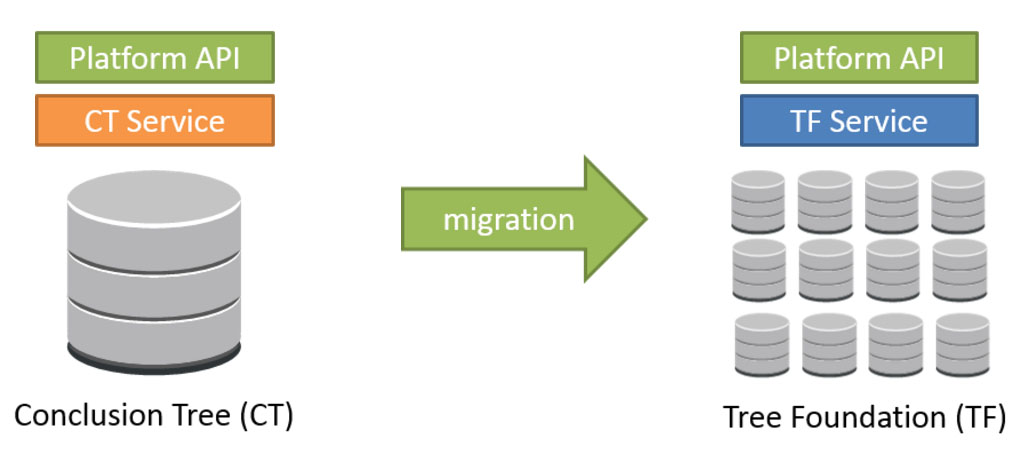
\includegraphics[scale=0.35]{04/treeFoundationDistributed}
        \centering
        \caption{Arquitectura \emph{Conclusion Tree} vs \emph{Tree Foundation}\label{fig:architecture}}
    \end{figure}

    Els beneficis esperats del canvi són un increment en l'escalabilitat del sistema, una millora eventual del rendiment, tot i que aquest no és l’objectiu principal durant les primeres fases d’implementació i finalment, una millor correlació entre el funcionament del sistema i com l'API accedeix a les dades.

    Addicionalment, el projecte canviarà part de la informació inclosa en els recursos accessibles a través de l'API.

    Un dels canvis que l’evolució de Tree Foundation pretén integrar i que avui en dia encara no es troba a producció, és integrar dins del recurs d’una persona, tota la informació que s’acostuma a consultar i que ara no contenia. Per exemple, les relacions familiars o les fonts de dades que verifiquen que la informació introduïda és correcta.

    Aquest canvi, pretén facilitar la navegació per les dades, evitant haver d’accedir a múltiples recursos per tal d’aconseguir tota la informació desitjada. D'aquesta forma, s'aconseguirà alliberar part la càrrega que suporta el sistema i millorar-ne, per tant, l'eficiència i disponibilitat. La figura~\ref{ref:resources} representa de forma visual el que aquest canvi implica en el recurs Persona.

    \begin{figure}[h]
        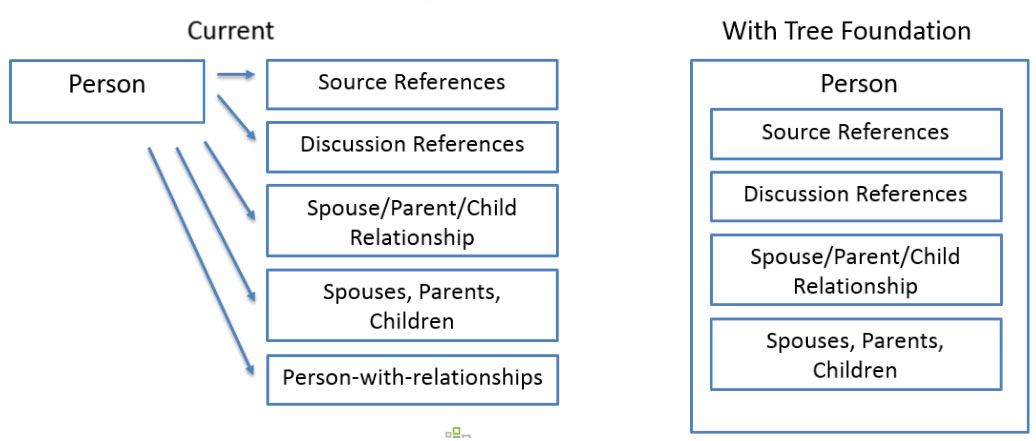
\includegraphics[scale=0.35]{04/resourceRellocation}
        \centering
        \caption{Relocalització d'informació sobre alguns recursos.\label{ref:resources}}
    \end{figure}

    Quan Tree Foundation va arribar a producció, només els recursos Source i Discussion, es trobaven incorporats dins del recurs Persona i els antics enllaços a aquesta informació quedaven obsolets. Més endavant, apuntant a mitjans d’Agost, s'espera que es realitzi el mateix canvi per les relacions familiars. La figura~\ref{ref:phase1}, mostra els canvis als quals ens estem referint.

    \begin{figure}[h]
        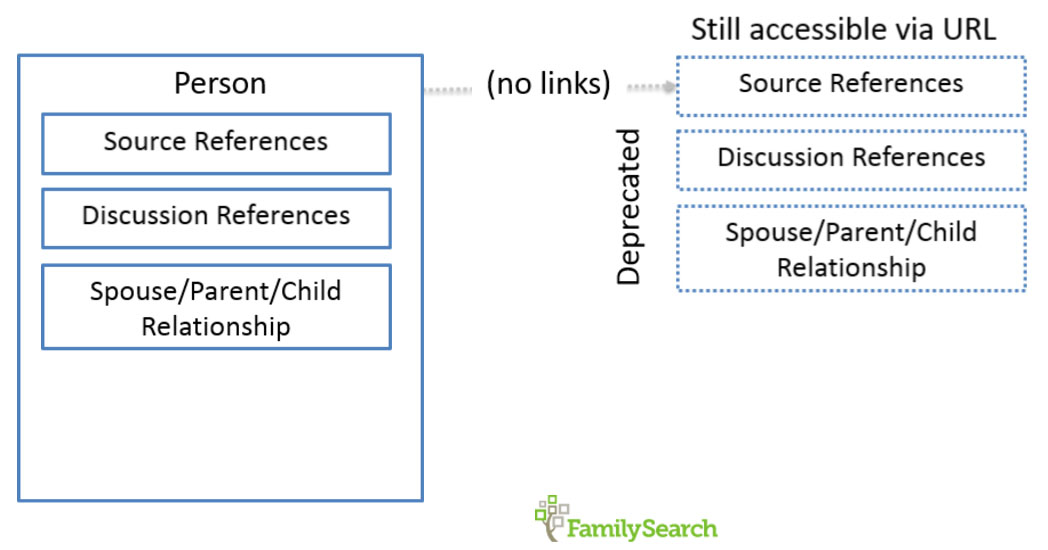
\includegraphics[scale=0.35]{04/phase1}
        \centering
        \caption{Localització dels recursos Discussió i Fonts de dades en la fase 1.\label{ref:phase1}}
    \end{figure}

    Tot i que el canvi és molt prometedor, cal tenir en compte que té el potencial de trencar part dels SDKs oficials i moltes de les aplicacions que tractin amb la versió antiga de l'API, de la mateixa forma que ja ho han fet les primeres versions de Tree Foundation arribades a producció.

    Per tant, caldrà estar al corrent de quan aquests canvis arriben a producció i de quan els SDKs oficials estaran preparats per ser utilitzats sense error, davant d'aquesta nova versió del back-end de FamilySearch.
